\chapter{Image Manipulation (2D)}

\section{Multiplanar Reconstruction}

When images are imported, InVesalius automatically shows its reconstruction
Multiplanar in the Axial, Sagittal and Coronal orientations, as well as a window for 3D manipulation.
See figure \ref{fig:mpr}.

\begin{figure}[!htb]
\centering
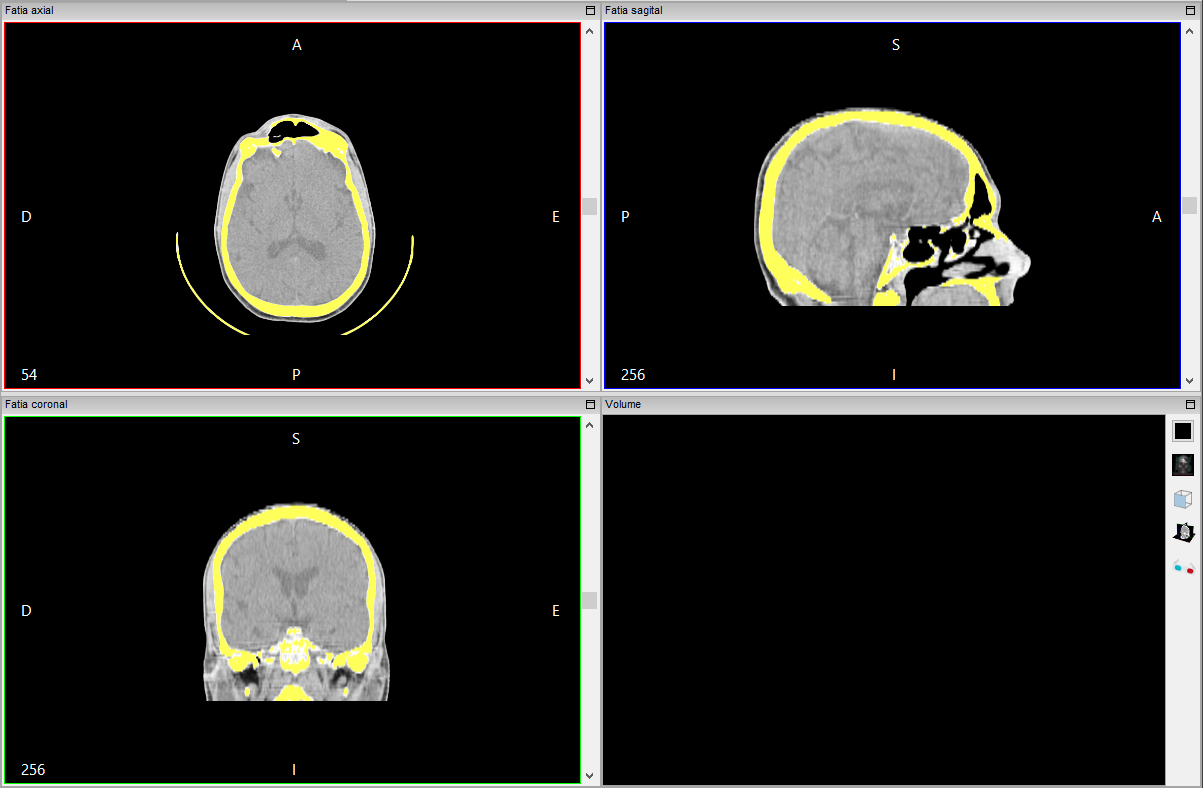
\includegraphics[scale=0.30]{multiplanar_mask_window_pt.png}
\caption{Multiplanar Reconstruction}
\label{fig:mpr}
\end{figure}

\newpage

In addition to creating a multiplanar reconstruction, InVesalius segments an image, highlighting, for example, soft tissue bones. The highlight is represented by the application of colors on a segmented structure, i.e., the colors forms a mask over an image highlighting the structure (figure \ref{fig:mpr}). This is discussed in more detail in the following chapters.


To hide the mask, use the data manager, located in the lower left corner
of the screen. Just choose the tab \textbf{Masks} and click \textbf{once} using the
\textbf{left} mouse buttom over the eye icon next to \textbf{"Mask 1"}. See figure
\ref{fig:ger_masc}.

\begin{figure}[!htb]
\centering
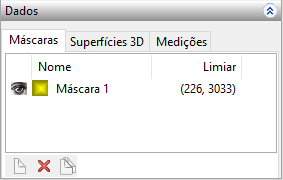
\includegraphics[scale=0.8]{data_mask_pt.png}
\caption{Mask manager}
\label{fig:ger_masc}
\end{figure}

The eye icon disappears, and the colors of the segmentation mask are hidden (figure
\ref{fig:mpr_sem_mask}).

\begin{figure}[!htb]
\centering
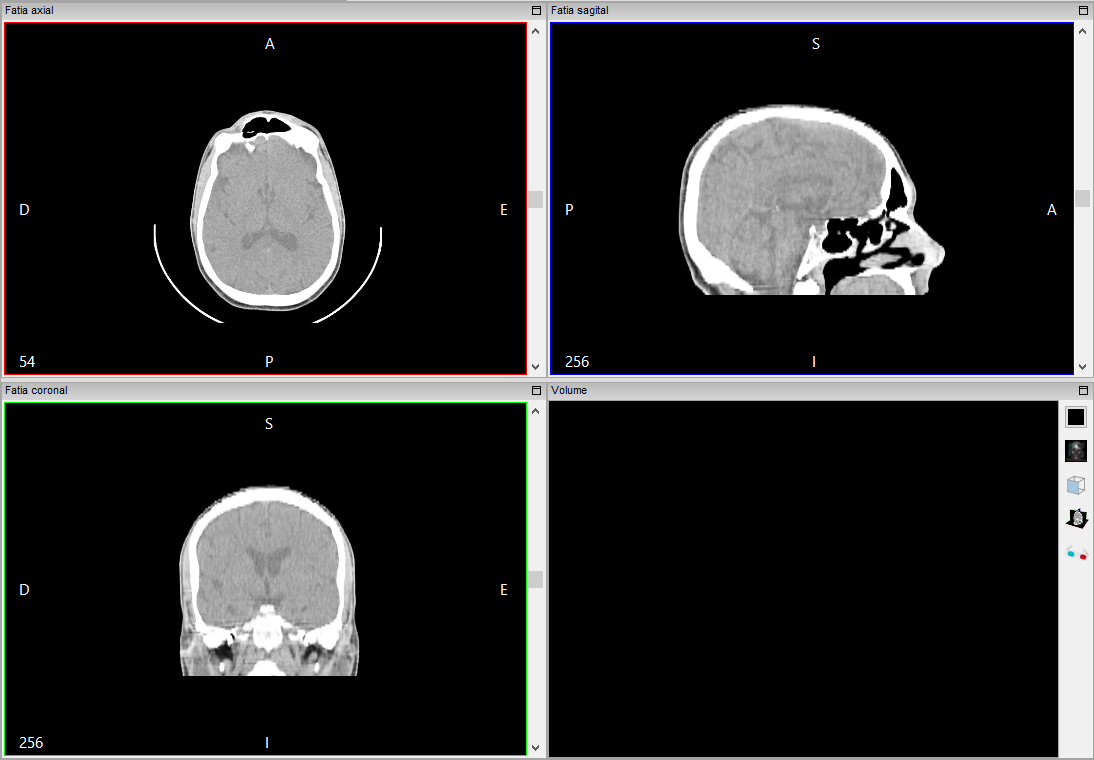
\includegraphics[scale=0.30]{multiplanar_window_pt.png}
\caption{Multiplanar reconstruction without segmentation mask}
\label{fig:mpr_sem_mask}
\end{figure}

\subsection{Axial orientation}

The axial orientation consists of cuts made transversal in relation to the region of interest, i.e. parallel cuts to the axial plane of the human body.
In figure \ref{fig:axial_corte}, an axial image of the skull region is displayed.

\begin{figure}[!htb]
\centering
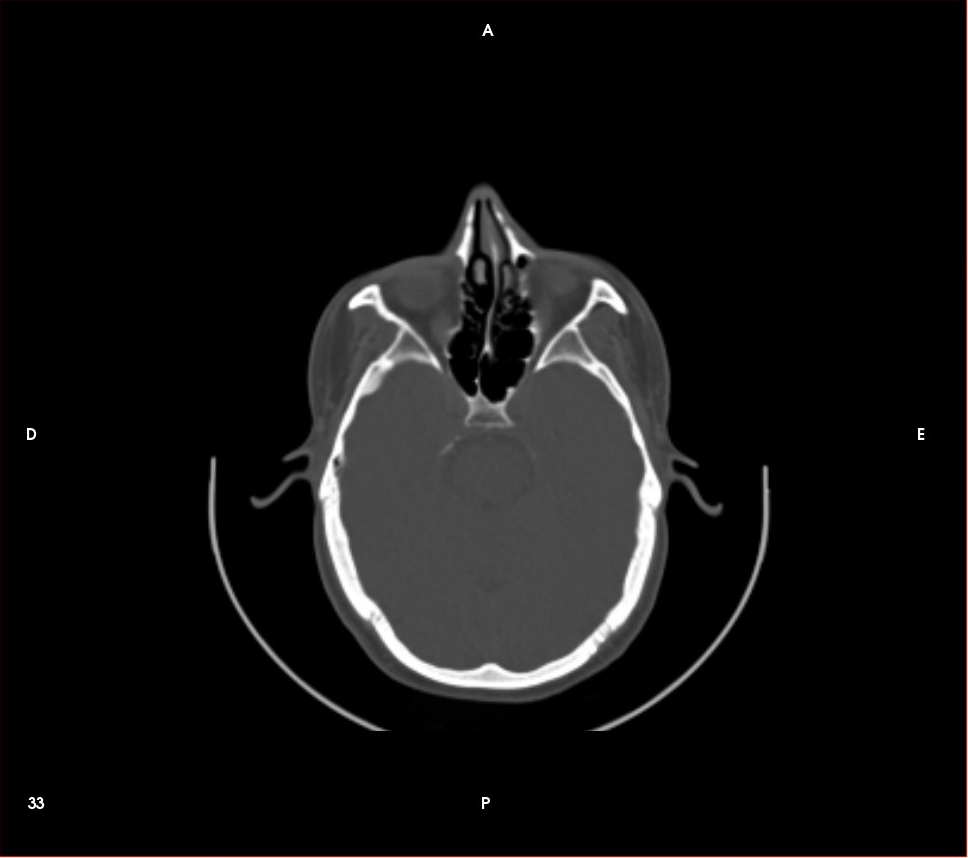
\includegraphics[scale=0.15]{axial.jpg}
\caption{Axial cut}
\label{fig:axial_corte}
\end{figure}

\subsection{Sagittal orientation}

The sagittal orientation consists of cuts made laterally in relation to the region of interest, i.e. parallel cuts to the sagittal plane of the human body, which divides it into the left and right portions.
In figure \ref{fig:sagital_slice}, a sagittal skull image is displayed.

\begin{figure}[!htb]
\centering
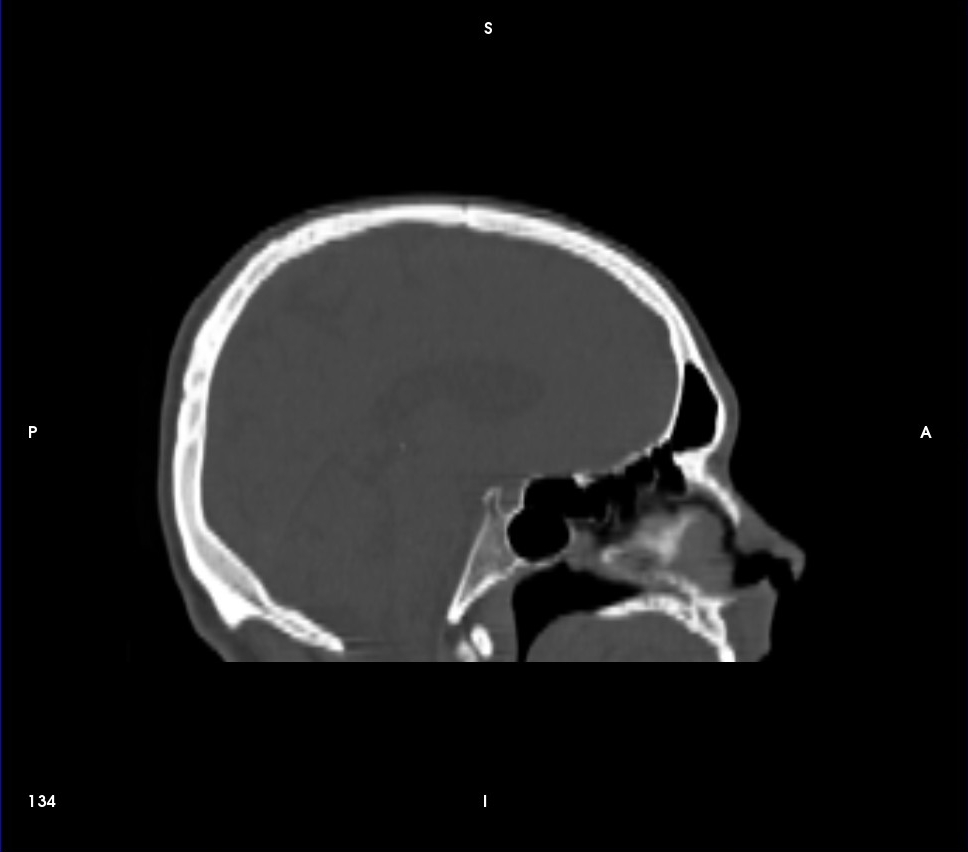
\includegraphics[scale=0.15]{sagital.jpg}
\caption{Sagittal cut}
\label{fig:sagital_slice}
\end{figure}

\newpage

\subsection{Coronal orientation}

The coronal orientation is composed of cuts parallel to the coronal plane, which divides the human body into ventral and dorsal halves.
In figure \ref{fig:coronal_slice} is displayed  a skull image in coronal orientation.

\begin{figure}[!htb]
\centering
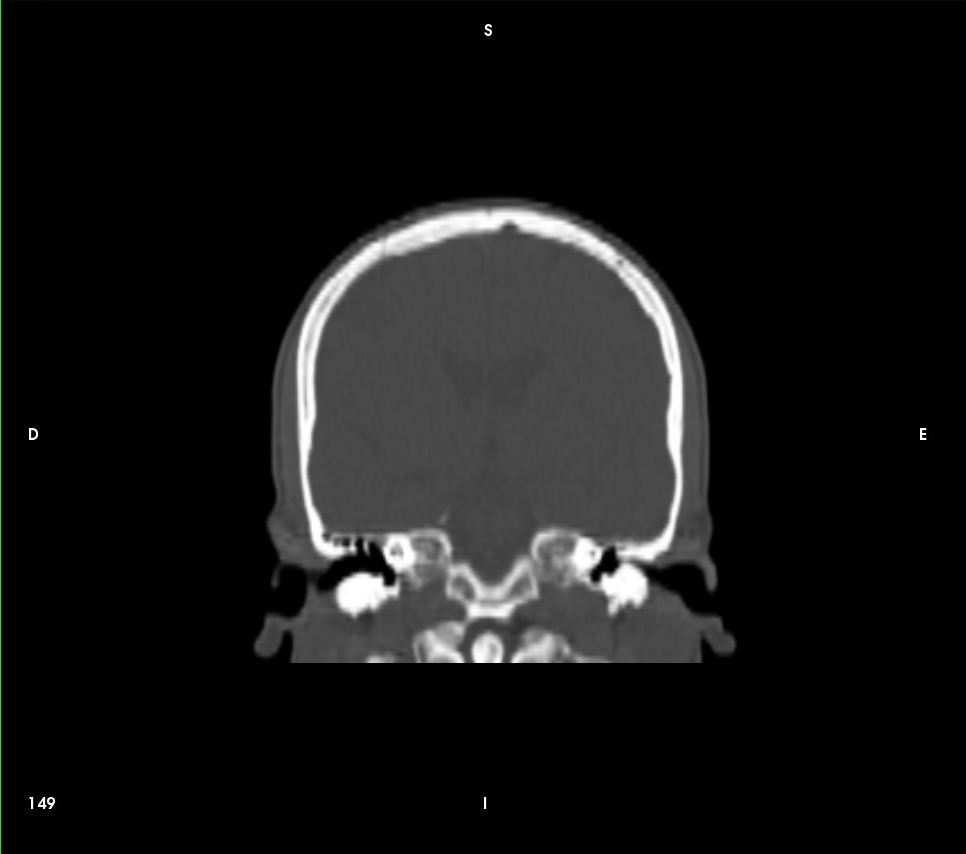
\includegraphics[scale=0.15]{coronal.jpg}
\caption{Coronal cut}
\label{fig:coronal_slice}
\end{figure}


\section{Correspondence between the axial, sagittal and coronal orientations}
\label{sec:corresp_all_orient}

To find out the common point of the images in differents orientations, simply activate the "Slices' cross intersection" feature with the shortcut icon located on the toolbar.
See figure \ref{fig:cross_icon}.

\begin{figure}[!htb]
\centering

\includegraphics[scale=1]{cross.png}
\caption{Shortcut to show common point between different orientations}
\label{fig:cross_icon}
\end{figure}

When the feature is fired, two cross segments that intersect perpendicularly are displayed on each image (figure \ref{fig:cross_all}). The intersection point of each pair of segments represents the common point between differents orientations.

\newpage

To modify the point, keep \textbf{pressed} the \textbf{left} mouse button and
\textbf{drag}. Automatically, the corresponding points will be updated in each image.

\begin{figure}[!htb]
\centering
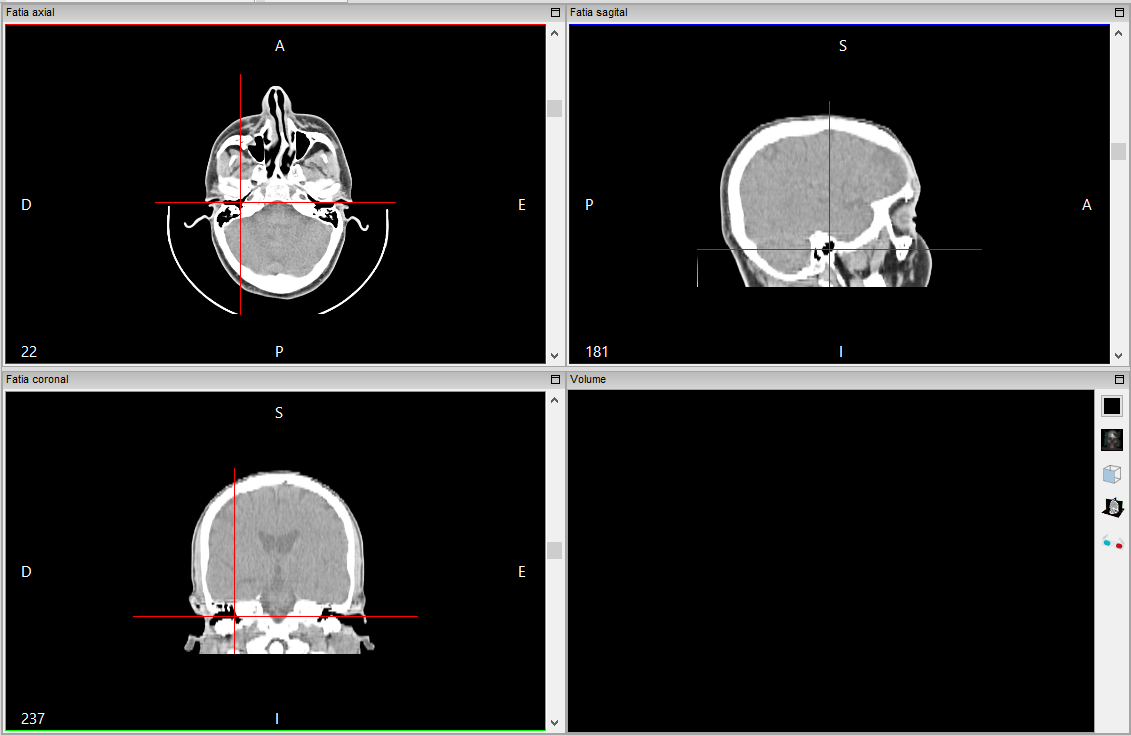
\includegraphics[scale=0.4]{multiplanar_window_cross_pt.png}
\caption{Common point between differents orientations}
\label{fig:cross_all}
\end{figure}

To disable the feature, simply click on the shortcut again (figure \ref{fig:cross_icon}). This feature can be used in conjunction with the slice editor (which will be discussed later).

\section{Interpolation}

By default the 2D images visualization are interpolated (figure~\ref{fig:interp}).a, to deactivate this feature, in menu press \textbf{View}, \textbf{Interpolated slices} (figure~\ref{fig:menu_interpoleted_image_pt}). In this way it will be possible to visualize each pixel individually as shown in the figure~\ref{fig:interp}.b.

\textbf{Note: This interpolation is for visualization purposes only, not directly influencing segmentation or 3D surface generation.}

\begin{figure}[!htb]
\centering
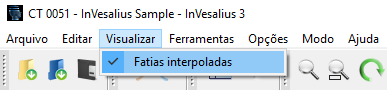
\includegraphics[scale=0.7]{menu_interpoleted_image_pt.png}
\caption{Menu to disable and enable interpolation}
\label{fig:menu_interpoleted_image_pt}
\end{figure}


\begin{figure}[!htb]
  \centering
  \subfloat[Interpolated]{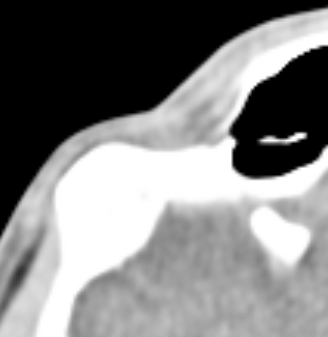
\includegraphics[width=0.4\textwidth]{axial_interpoleted.png}}  \qquad
  \subfloat[Non-interpolated]{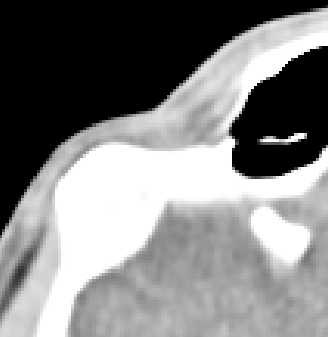
\includegraphics[width=0.4\textwidth]{axial_not_interpoleted.png}}
  \hfill
  \caption{Interpolated and non-interpolated image visualization.}
  \label{fig:interp}
\end{figure}

\section{Move}

To move an image on the screen, the toolbar's "Move" shortcut icon can be used (figure
\ref{fig:move_icon}). Click on the icon to activate the feature and then with the \textbf{left} mouse button on the image, \textbf{drag} it to the desired direction. The figure \ref{fig:move_img} shows a displaced (moved) image.

\begin{figure}[!htb]
\centering

\includegraphics[scale=0.25]{tool_translate_original.png}
\caption{Shortcut to move images}
\label{fig:move_icon}
\end{figure}

\begin{figure}[!htb]
\centering
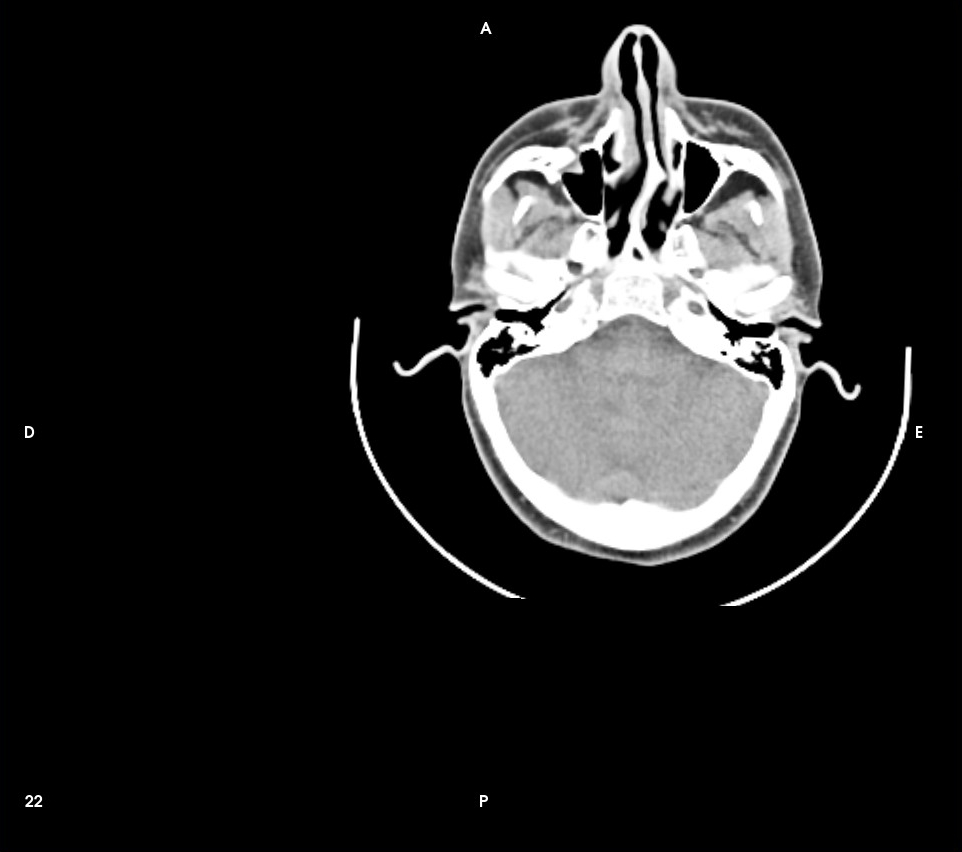
\includegraphics[scale=0.25]{axial_pan.jpg}
\caption{Displaced image}
\label{fig:move_img}
\end{figure}

\section{Rotate}

The image rotation can be activated by the toolbar's "Rotate" shortcut icon (figure \ref{fig:rot_icon}). To rotate an image, click on the icon and then with the \textbf{left} mouse button press on the image, \textbf{drag} clockwise or anticlockwise, depending on the desired direction of rotation.

\begin{figure}[!htb]
\centering

\includegraphics[scale=0.25]{tool_rotate_original.png}
\caption{Shortcut to rotate images}
\label{fig:rot_icon}
\end{figure}

\begin{figure}[!htb]
\centering
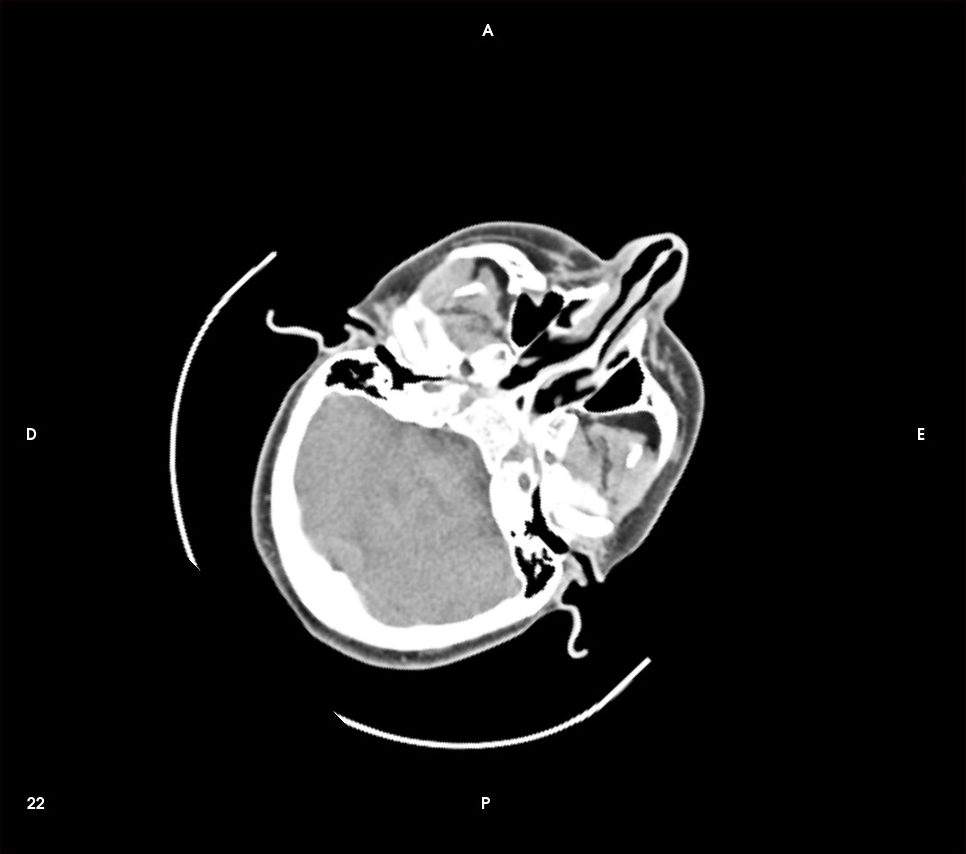
\includegraphics[scale=0.25]{axial_rotate.jpg}
\caption{Rotated image}
\label{fig:rotate_all}
\end{figure}

\section{Zoom}

In InVesalius, there are different ways to enlarge an image. You can maximize the desired orientation window, apply zoom directly to the image, or select the region of the image to enlarge.

\subsection{Maximizing orientation windows}

As we already know, the main InVesalius window is divided into 4 subwindows: axial, sagittal, coronal and 3D. Each of these can be maximized to occupy the entire area of the main window. To do this, simply \textbf{left} mouse click on the subwindow icon located in the \textbf{upper right corner} (figure \ref{fig:maximize_window}). To restore a maximized window to its previous size, simply click the icon again.

\begin{figure}[!htb]
\centering
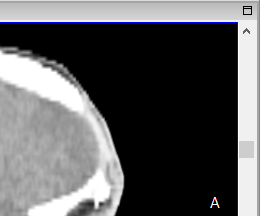
\includegraphics[scale=0.6]{maximize_sagital_mpr.png}
\caption{Detail of a sub-window (Note the maximize icon in the upper right corner)}
\label{fig:maximize_window}
\end{figure}

\subsection{Enlarging or reducing an image}

To enlarging or reducing an image, click on the zoom shortcut icon in the toolbar (figure \ref{fig:zoom_icon}). Hold down the \textbf{left} mouse button on the image and \textbf{drag} the mouse to \textbf{top} if you want to enlarge it, or \textbf{down}, if you want to reduce it.

\begin{figure}[!htb]
\centering

\includegraphics[scale=0.25]{tool_zoom_original.png}
\caption{Zoom shortcut}
\label{fig:zoom_icon}
\end{figure}

%\begin{figure}[!htb]
%\centering
%\includegraphics[scale=0.2]{ScreenHunter_76Dec311201_.jpg}
%\caption{Imagem com \textit{Zoom} aplicado}
%\label{fig:zoom_}
%\end{figure}

\subsection{Enlarging an Image Area}

To enlarging a certain image area, click on the "Zoom based on selection" icon in the toolbar (figure \ref{fig:zoom_icon_loc}). Position the mouse pointer at the start position of the selection, click and hold the \textbf{left} mouse button and \textbf{drag} it to the end selection position, forming a rectangle (figure \ref{fig:zoom_select}). Once the left mouse button is released, the zoom operation will be applied to the selected region (figure \ref{fig:zoom_applied}).

\begin{figure}[!htb]
\centering

\includegraphics[scale=0.25]{tool_zoom_select_original.png}
\caption{Zoom based on selection shortcut}
\label{fig:zoom_icon_loc}
\end{figure}

\begin{figure}[!htb]
\centering
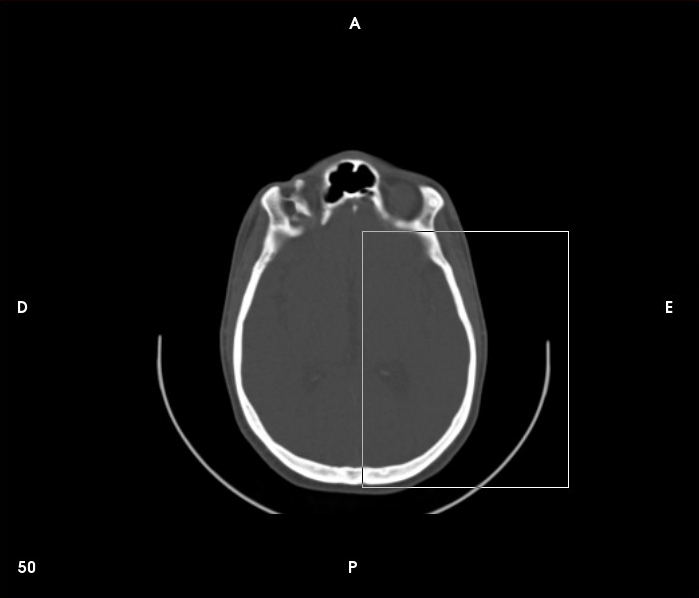
\includegraphics[scale=0.25]{tool_zoom_select_image.jpg}
\caption{Area selected for zoom}
\label{fig:zoom_select}
\end{figure}

\begin{figure}[!htb]
\centering
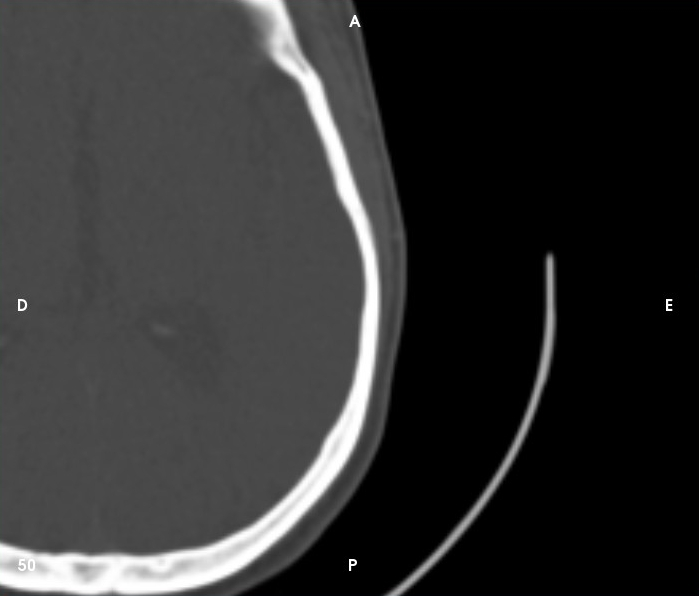
\includegraphics[scale=0.25]{tool_image_with_zoom.jpg}
\caption{Enlarged Image}
\label{fig:zoom_applied}
\end{figure}


\section{Brilho e contraste (Janelas)}
\label{sec:ww_wl}

Para melhorar a visualização das imagens, podemos utilizar o recurso de \textit{window width} e
\textit{window level}, popularmente conhecido por "brilho e contraste" ou "janela" (para radiologistas). 
Com esse recurso, é possível definir a faixa da escala de cinza (\textit{window level}) e a
largura dessa faixa (\textit{window width}) que serão usadas para exibir as imagens.

O recurso pode ser acionado pelo ícone do atalho "Contraste" na barra de ferramentas. Veja a figura \ref{fig:window_level_shortcut}.

\begin{figure}[!htb]
\centering

\includegraphics[scale=0.70]{tool_contrast_original.png}
\caption{Atalho de brilho e contraste}
\label{fig:window_level_shortcut}
\end{figure}

Para aumentar o brilho, mantenha o botão \textbf{esquerdo} do mouse pressionado e o \textbf{arraste} na 
horizontal para a direita. Para diminuir o brilho, basta arrastar o mouse para a esquerda. O contraste
pode ser alterado arrastando o mouse (com o botão \textbf{esquerdo} pressionado) na vertical: para cima
para aumentar, ou para baixo para diminuir o contraste.

Para desabilitar o recurso, clique novamente sobre o ícone do atalho (figura \ref{fig:window_level_shortcut}).

É possível utilizar padrões pré-definidos de brilho e contraste. A tabela \ref{tab:window_level} relaciona
alguns tipos de tecido com os respectivos valores de brilho e contraste da imagem. Para usar um padrão
pré-definido, posicione o cursor do mouse sobre a imagem e clique com o botão \textbf{direito} para abrir um
menu de contexto sobre ela. Quando o menu se abrir, selecione a entrada \textbf{Brilho e Contraste} e, em
seguida, clique sobre a opção pré-definida, de acordo com o tipo de tecido, como mostra a figura
\ref{fig:window_level}.


\begin{figure}[!htb]
\centering
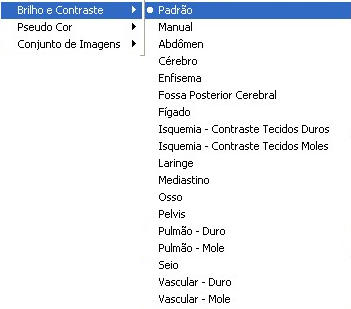
\includegraphics[scale=0.40]{menu_window_and_level_pt.png}
\caption{Menu de contexto para seleção de brilho e contraste}
\label{fig:window_level}
\end{figure}

\begin{table}[h]
\centering
\caption{Valores de brilho e contraste para alguns tecidos}
\begin{tabular}{lcc}\\
\hline % este comando coloca uma linha na tabela
Tecido & Brilho & Contraste\\
\hline
\hline
Padrão & Exame & Exame\\
Manual & Alterado & Alterado\\
Abdômen & 350 & 50 \\
Cérebro & 80 & 40\\
Enfisema & 500 & -850\\
Fossa Posterior Nasal & 120 & 40\\
Fígado & 2000 & -500\\
Isquemia - Contraste Tecidos Duros & 15 & 32\\
Isquemia - Contraste Tecidos Moles & 80 & 20\\
Laringe & 180 & 80\\
Mediastino & 350 & 25\\
Osso & 2000 & 300\\
Pélvis & 450 & 50\\
Pulmão Duro & 1000 & -600\\
Pulmão Mole & 1600 & -600\\
Seio & 4000 & 400\\
Vascular - Duro & 240 & 80\\
Vascular - Mole & 680 & 160\\
\hline
\end{tabular}
\label{tab:window_level}
\end{table} 

\begin{figure}
  \centering
  \subfloat[Osso]{\label{fig:contrast_bone}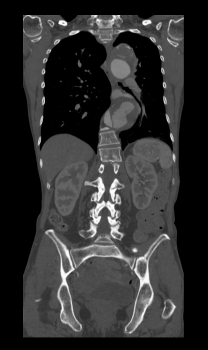
\includegraphics[width=0.4\textwidth]{contraste_osso}}                
  \subfloat[Pulmão]{\label{fig:contrast_isq}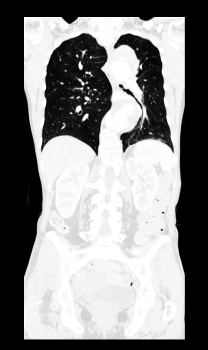
\includegraphics[width=0.4\textwidth]{contraste_pulmao}}
  \caption{Diferentes tipos de brilho e constraste}
  \label{fig:two_window_level}
\end{figure}


\section{Pseudocor}

Outro recurso para melhorar a visualização das imagens são as pseudocores. Elas substituem os níveis
de cinza por cores, ou pelos níveis de cinza invertidos. Nesse último caso, regiões da imagem que
antes eram mais claras se tornam mais escuras e vice-versa.

Para alterar a visualização usando uma pseudocor, posicione o cursor do mouse sobre a imagem e clique
com o botão \textbf{direito} para abrir um menu de contexto sobre ela. Quando o menu se abrir,
selecione a entrada \textbf{Pseudocor} e, em seguida, clique sobre a opção de pseudocor desejada, como
mostra a figura \ref{fig:pseudo_color}.

\begin{figure}[H]
\centering
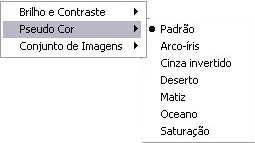
\includegraphics[scale=0.40]{pseudo_menu_pt.png}
\caption{Pseudo Cor}
\label{fig:pseudo_color}
\end{figure}

As figuras de \ref{fig:image_default} a \ref{fig:image_saturation} exemplificam as diversas opções de
pseudocor disponíveis.\\

\begin{figure}[H]
\centering
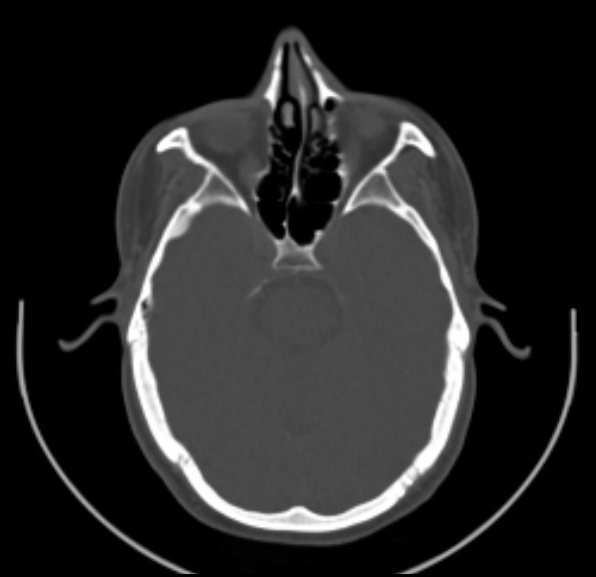
\includegraphics[scale=0.30]{pseudo_default.jpg}
\caption{Padrão}
\label{fig:image_default}
\end{figure}

\begin{figure}[H]
\centering
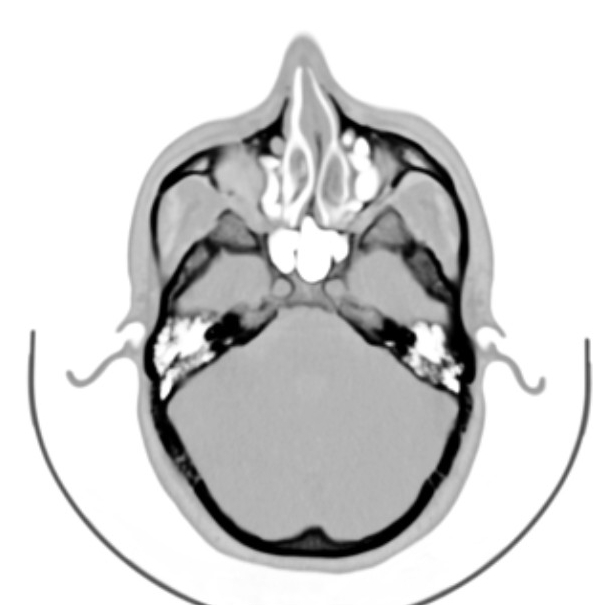
\includegraphics[scale=0.30]{pseudo_inverse.jpg}
\caption{Imagem Cinza Invertido}
\label{fig:image_inverted}
\end{figure}

\begin{figure}[H]
\centering
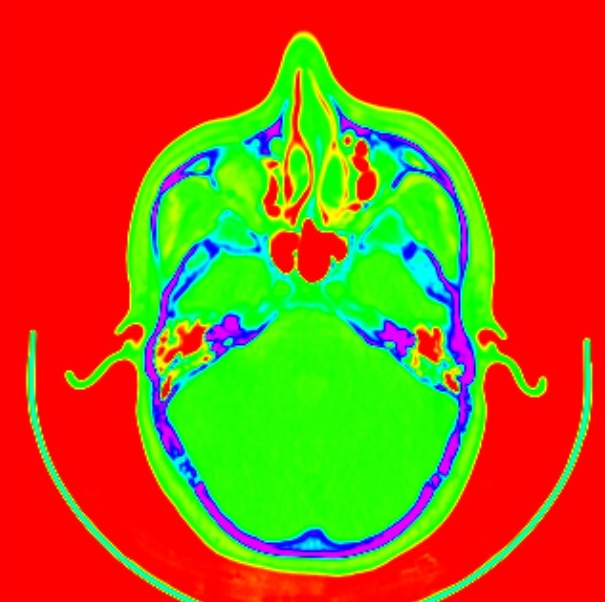
\includegraphics[scale=0.30]{pseudo_rainbow.jpg}
\caption{Arco-íris}
\label{fig:image_arc}
\end{figure}

\begin{figure}[H]
\centering
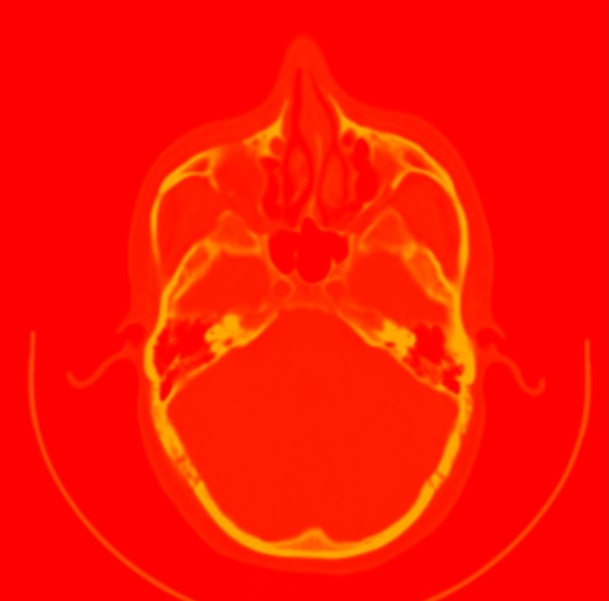
\includegraphics[scale=0.30]{pseudo_desert.jpg}
\caption{Deserto}
\label{fig:image_desert}
\end{figure}

\begin{figure}[H]
\centering
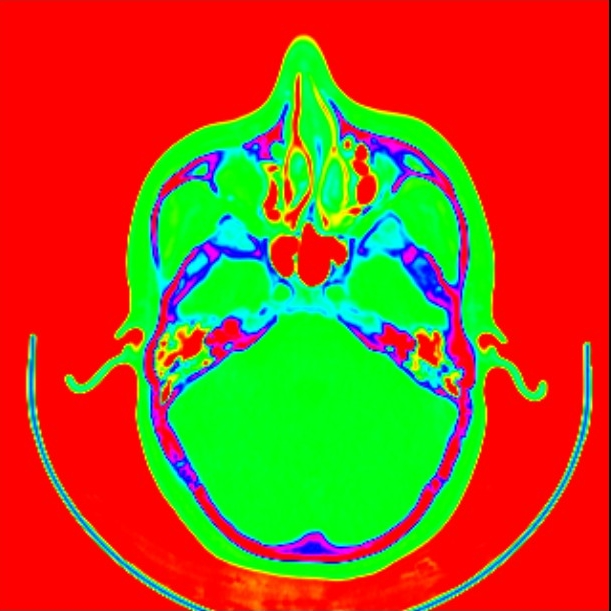
\includegraphics[scale=0.30]{pseudo_hue.jpg}
\caption{Matiz}
\label{fig:image_matiz}
\end{figure}

\begin{figure}[H]
\centering
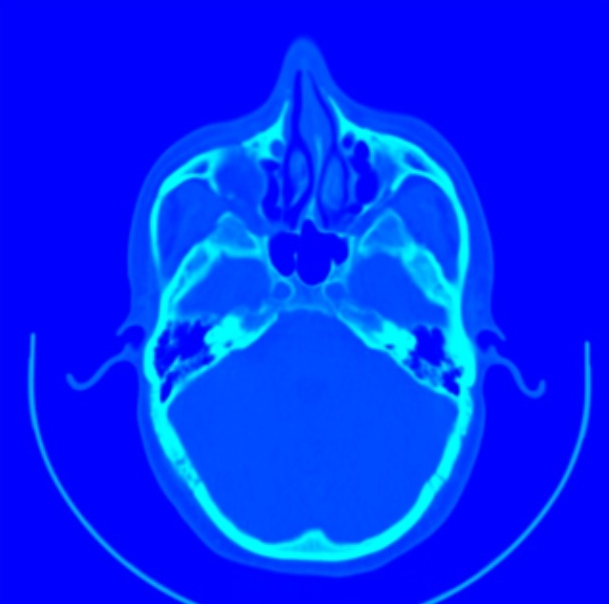
\includegraphics[scale=0.30]{pseudo_ocean.jpg}
\caption{Oceano}
\label{fig:image_ocean}
\end{figure}

\begin{figure}[H]
\centering
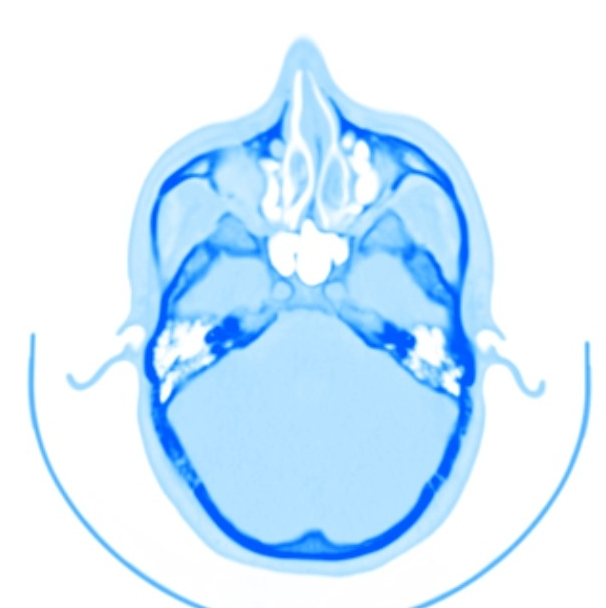
\includegraphics[scale=0.30]{pseudo_saturation.jpg}
\caption{Saturação}
\label{fig:image_saturation}
\end{figure}

\newpage

\section{Tipo de projeção}

É possível alterar o tipo de projeção das imagens 2D a serem visualizadas, além do modo normal, o InVesalius dispõe de seis tipos de projeções que podem serem acessadas da seguinte forma: Possicione o cursor do mouse sobre a imagem e clique com o botão \textbf{direito} para abrir um menu de contexto sobre ela. Quando o menu se abrir, selecione a entrada tipo de projeção e, em seguida, clique sobre a opção de pseudocor desejada, como mostra a figura~\ref{fig:menu_proj}.

\begin{figure}[H]
\centering
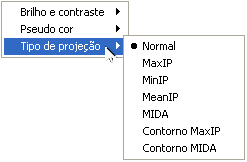
\includegraphics[scale=0.60]{menu_projection_pt.png}
\caption{Menu de Tipo de projeção}
\label{fig:menu_proj}
\end{figure}

\subsection{Normal}

O modo normal é a visualização padrão, ou seja, sem nenhum tipo de projeção, da maneira em que a imagem foi adquirida ou customizada previamente seja com brilho e contraste ou pseudocor. Exemplificamos na figura~\ref{fig:proj_normal}.

\begin{figure}[H]
\centering
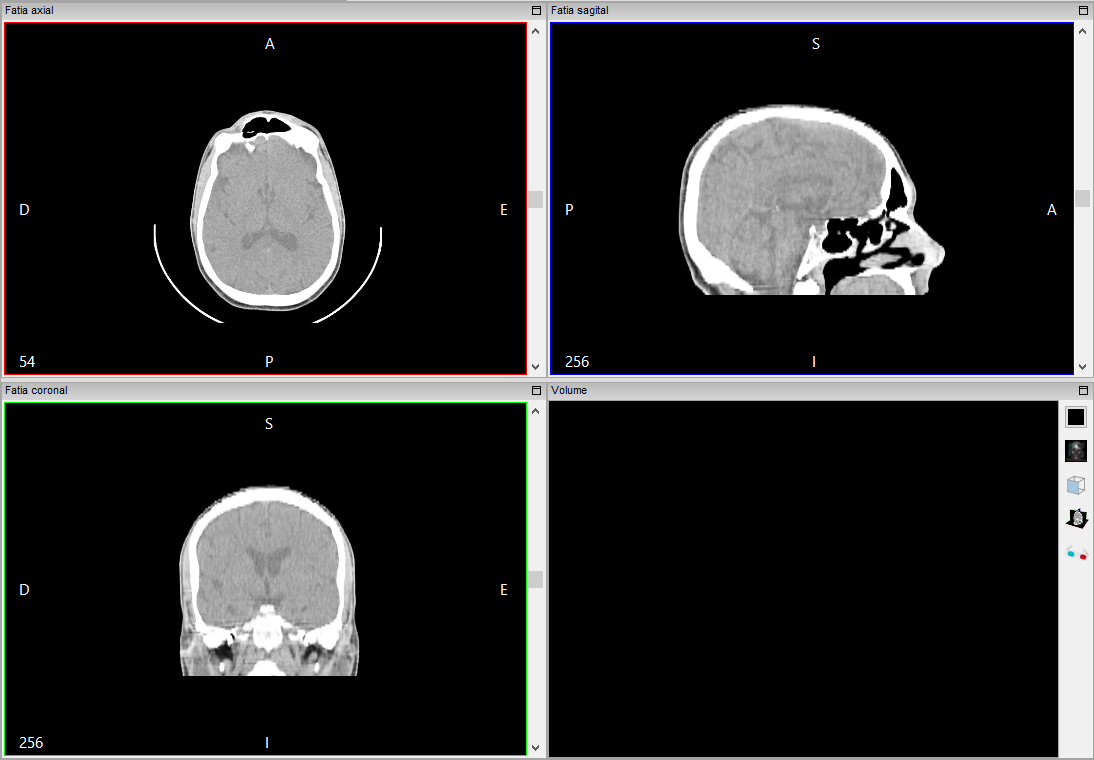
\includegraphics[scale=0.40]{multiplanar_window_pt.png}
\caption{Projeção normal}
\label{fig:proj_normal}
\end{figure}

\subsection{MaxIP}
\label{sec:max_ip}
MaxIP também é conhecido como MIP (\textit{Maximum Intensity Projection}), o método seleciona somente os voxels que possuem intensidade máxima entre os visitados como mostra a figura~\ref{fig:proj_maxip}. De acordo com a quantidade ou "profundidade" do MaxIP cada voxel é visitado em ordem de sobreposição, por exemplo, para selecionar MaxIP do pixel $(0,0)$ composto por 3 fatias é necessário visitar o pixel $(0,0)$ das fatias $(1,2,3)$ e selecionar o maior valor.

\begin{figure}[H]
\centering
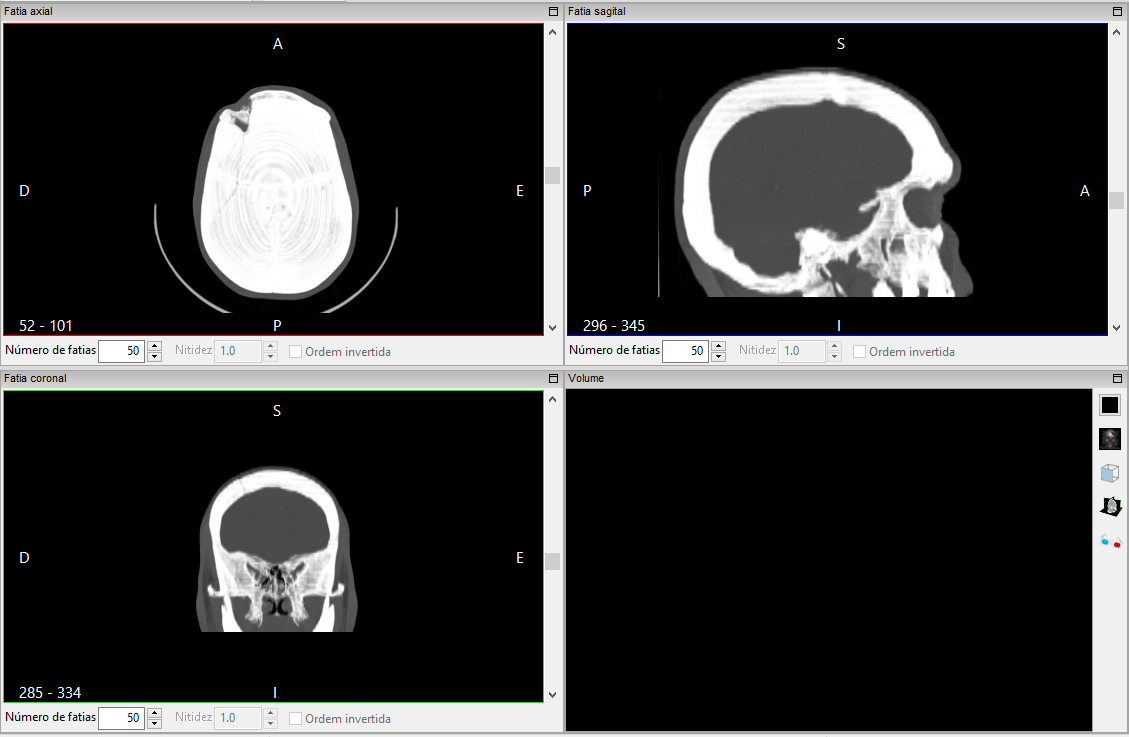
\includegraphics[scale=0.40]{multiplanar_window_maxip_pt.png}
\caption{Projeção MaxIP ou MIP}
\label{fig:proj_maxip}
\end{figure}

Como mostra a figura~\ref{fig:proj_maxip_qtd}, a quantidade de imagens que irá compor o MaxIP é setada no inferior da imagem de cada orientação.

\begin{figure}[H]
\centering
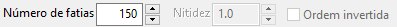
\includegraphics[scale=0.80]{multiplanar_window_maxip_number_pt.png}
\caption{Seleção da quantidade de imagens que compõe o MaxIP ou MIP}
\label{fig:proj_maxip_qtd}
\end{figure}

\subsection{MinIP}

Ao contrário do MaxIP, o MinIP (\textit{Minimun Intensity Projection}) seleciona somente os voxels que possuem internsidade minima entre os visitados, apresentamos na figura~\ref{fig:proj_minIP} um exemplo. A seleção da quantidade de imagens que irá compor a projeção é feita no inferior da imagem de cada orientação como mostra a figura~\ref{fig:proj_maxip_qtd}.

\begin{figure}[H]
\centering
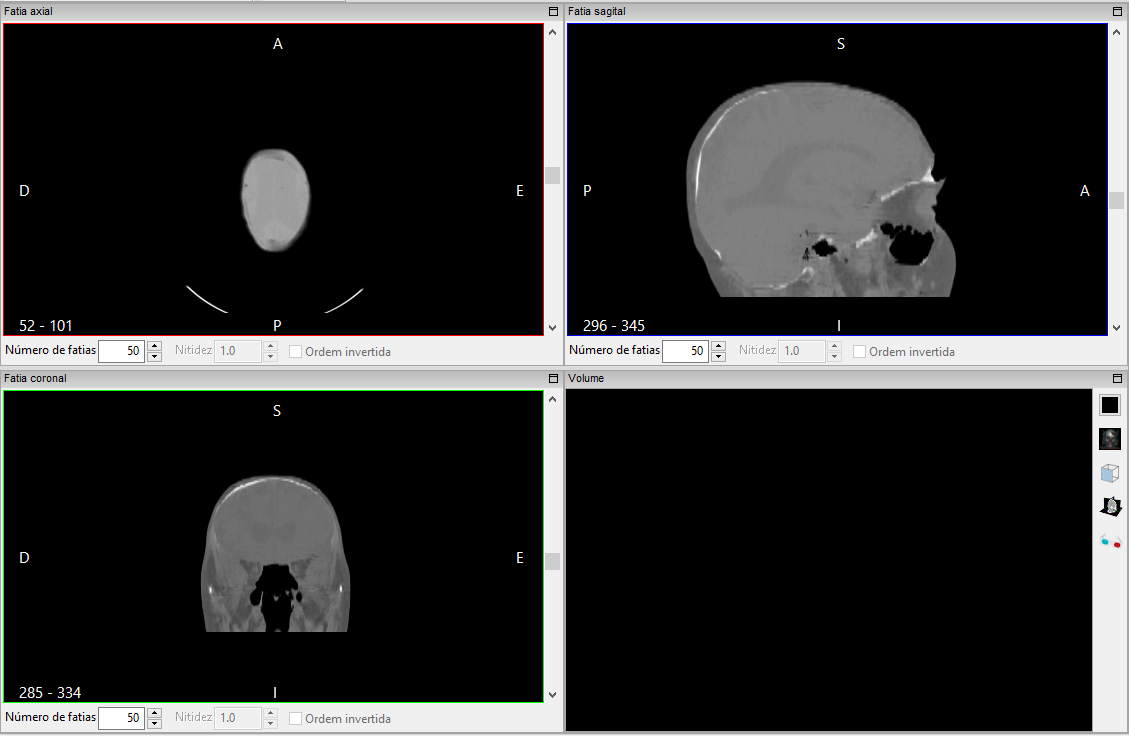
\includegraphics[scale=0.40]{multiplanar_window_minip_pt.png}
\caption{Projeção MinIP}
\label{fig:proj_minIP}
\end{figure}

\subsection{MeanIP}
A técnica MeanIP (\textit{Mean Intensity Projection}) que é mostrada na figura~\ref{fig:proj_meanIP} compõe a projeção realizando a média dos voxels visitados. Os voxels são visitados da mesma forma dos métodos MaxIP e MinIP. Também é possível definir quantas imagens irão compor a projeção no inferior da imagem de cada orientação como é mostrada na figura~\ref{fig:proj_maxip_qtd}.

\begin{figure}[H]
\centering
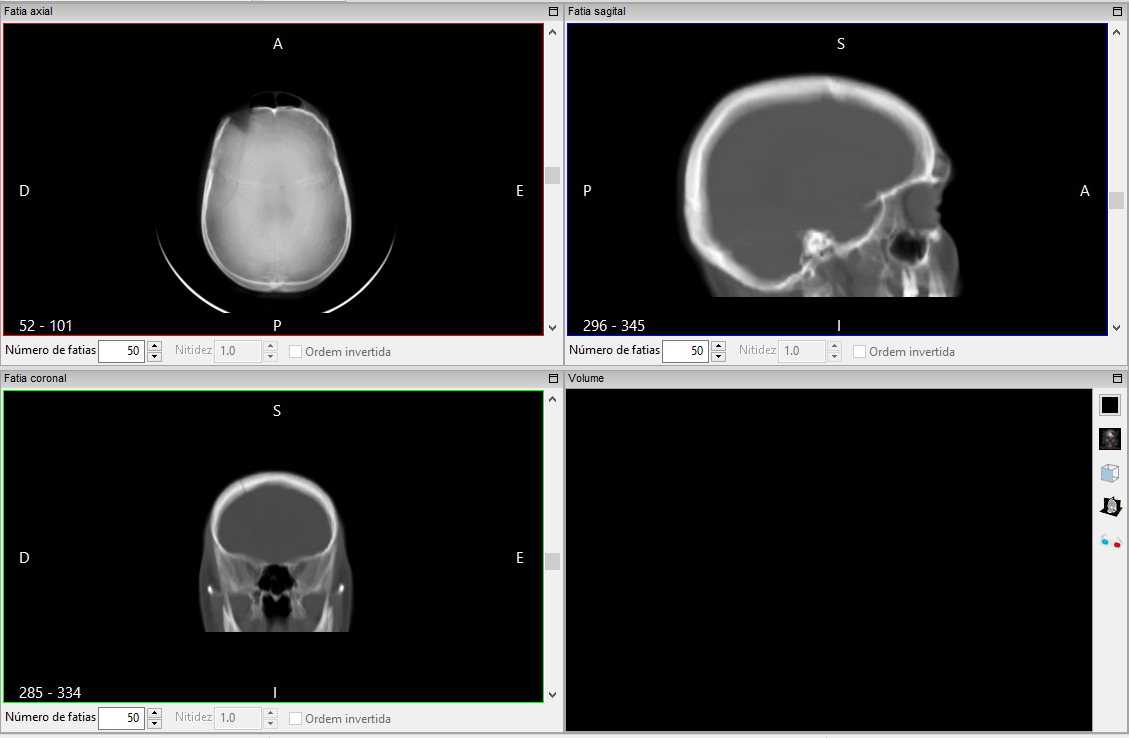
\includegraphics[scale=0.40]{multiplanar_window_mean_pt.png}
\caption{Projeção MeanIP}
\label{fig:proj_meanIP}
\end{figure}

\subsection{MIDA}
\label{sub:mida}
A técnica MIDA (\textit{Maximum Intensity Difference Accumulation}) projeta uma imagem levando em consideração somente os voxels que possuem valores máximos locais. A partir de cada pixel da tela é simulado um raio em direção ao volume, cada voxel é interceptado por cada um destes raios chegando até o final do volume, cada um desses voxels visitados tem o seu valor acumulado, mas são levados em consideração somente se o valor for maior que os valores já visitados anteriormente. A exemplo do MaxIP, é possível selecionar quantas imagens serão utilizadas para acumular os valores. Apresentamos na figura~\ref{fig:proj_MIDA} um exemplo de projeção MIDA.  

\begin{figure}[H]
\centering
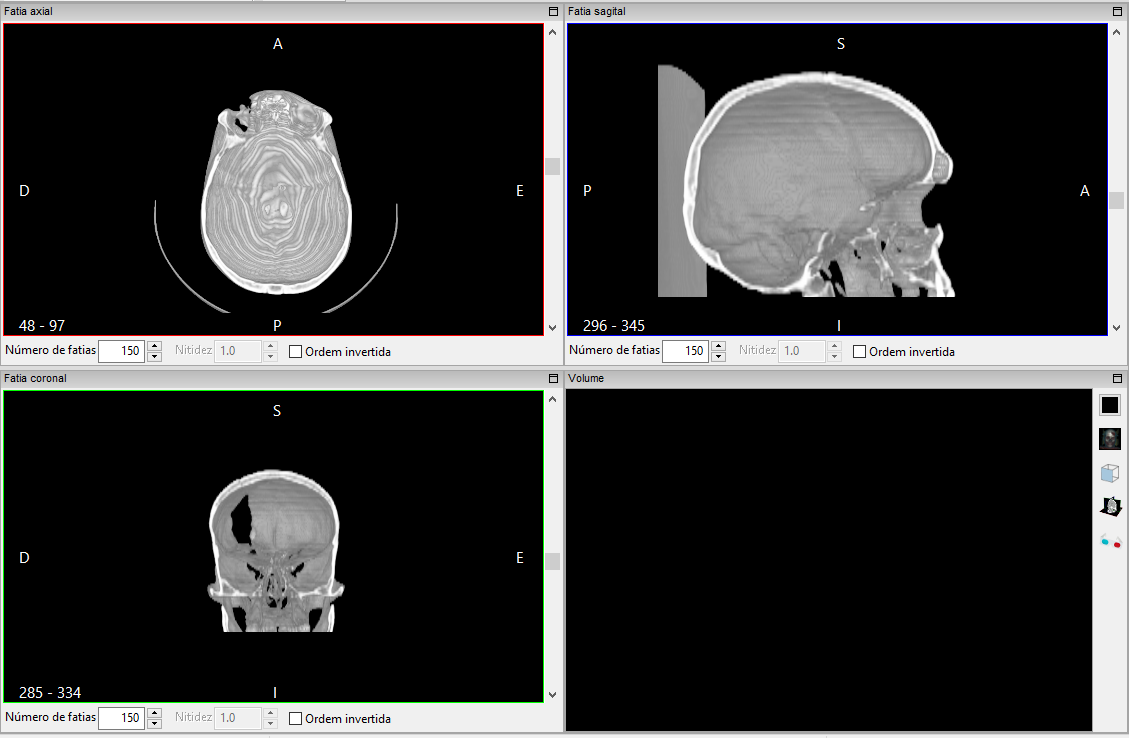
\includegraphics[scale=0.40]{multiplanar_window_mida_pt.png}
\caption{Projeção MIDA}
\label{fig:proj_MIDA}
\end{figure}

Como mostra a figura~\ref{fig:proj_MIDA_inv}, é possível inverter a ordem que os voxels são visitados, bastando selecionar a opção \textbf{Ordem invertida} no canto inferior da tela.

\begin{figure}[H]
\centering
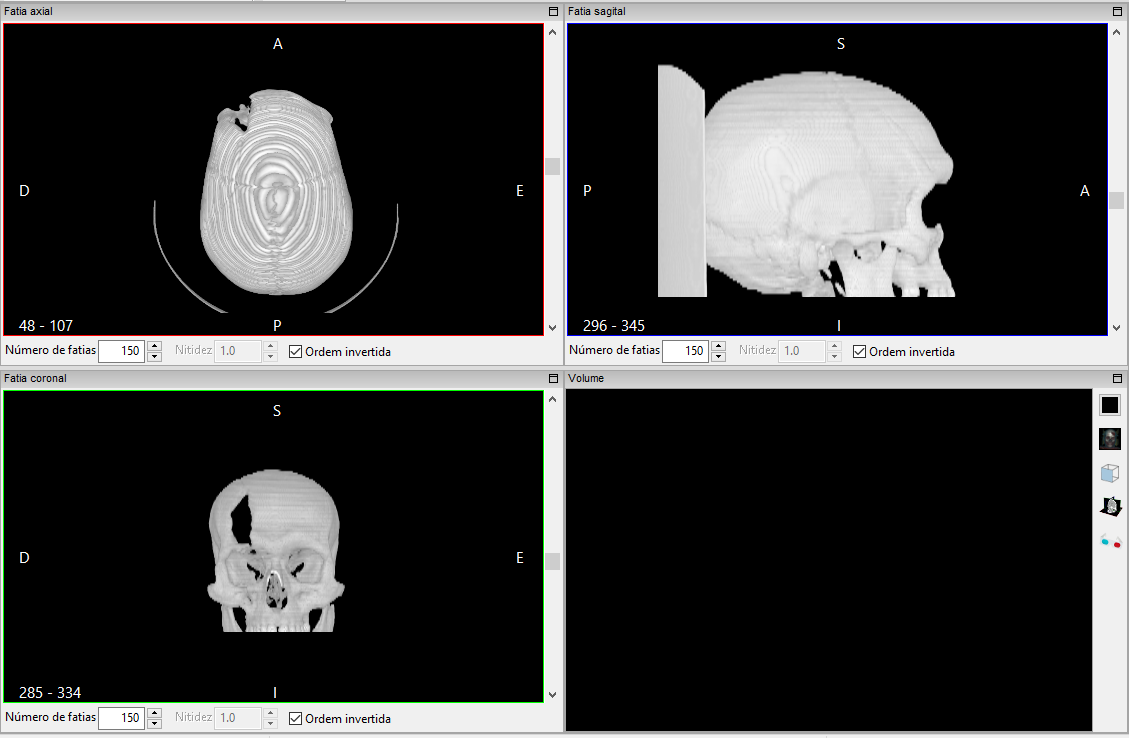
\includegraphics[scale=0.40]{multiplanar_window_mida_inverted_pt}
\caption{Projeção MIDA em ordem invertida}
\label{fig:proj_MIDA_inv}
\end{figure}

\subsection{Contorno MaxIP}

Compõe a projeção 2D do conjunto de imagens que contém o volume usando a técnica \textit{Contour MaxIP}. A técnica consiste em visualizar contornos presentes na projeção gerada com a técnica MaxIP(\ref{sec:max_ip}). Um exemplo é apresentado na figura~\ref{fig:proj_contorno_maxip}.

\begin{figure}[H]
\centering
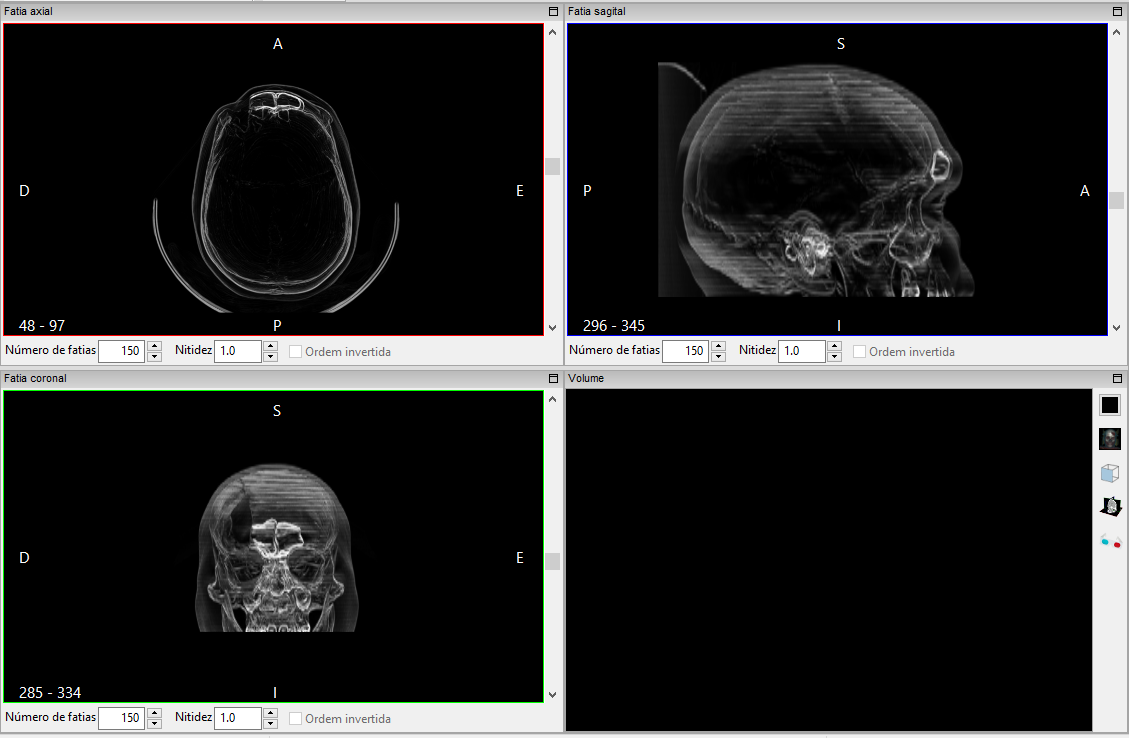
\includegraphics[scale=0.40]{multiplanar_window_contour_maxip_pt.png}
\caption{Projeção de Contorno MaxIP}
\label{fig:proj_contorno_maxip}
\end{figure}

\subsection{Contorno MIDA}

Compõe a projeção 2D do conjunto de imagens que contém o volume usando a técnica \textit{Contour MIDA}. A técnica consiste em visualizar contornos presentes na projeção gerada com a técnica MIDA(\ref{sub:mida}). A exemplo do MIDA é possível inverter a ordem que o volume é visitado. Exemplificamos na figura~\ref{fig:proj_contorno_mida}.

\begin{figure}[H]
\centering
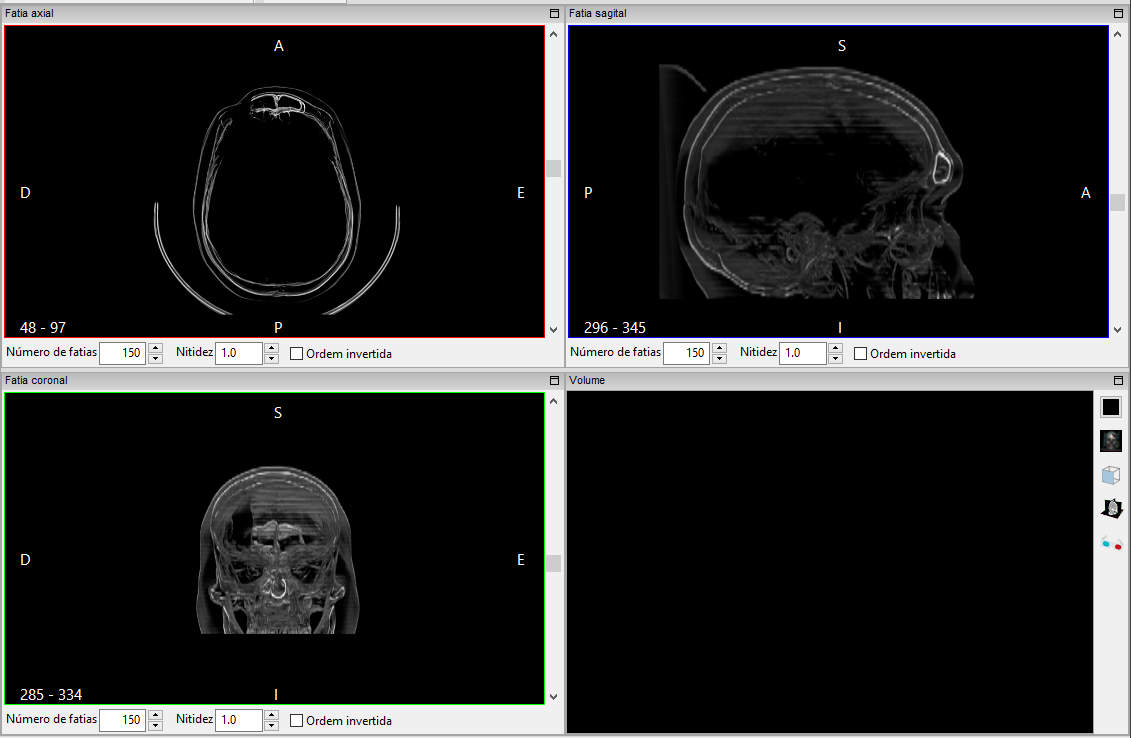
\includegraphics[scale=0.40]{multiplanar_window_contour_mida_pt.png}
\caption{Projeção de Contorno MIDA}
\label{fig:proj_contorno_mida}
\end{figure}